\documentclass[12pt,english]{amsart}
\usepackage[utf8]{inputenc}
\usepackage{fontenc}
\usepackage{mathtools}
\usepackage{amscd, bbold}
\usepackage{amsmath,amsthm,amssymb,amsfonts,mathrsfs}
\usepackage[pdftex,bookmarks,colorlinks,breaklinks]{hyperref}
\usepackage{comment}
\usepackage{graphicx}
\setlength{\parindent}{0pt}
\usepackage[top=3cm,bottom=3cm,right=2.3cm,left=2.3cm,twoside=false]{geometry}

\hypersetup{linkcolor=blue,citecolor=red,filecolor=dullmagenta,urlcolor=blue}
%\usepackage{verbatim}
%\usepackage{showkeys}

%\newtheorem{theorem}{Theorem}[section]
%\newtheorem{definition}{Definition}
%\newtheorem{lemma}[theorem]{Lemma}
%\newtheorem{proposition}[theorem]{Proposition}
%\newtheorem{corollary}[theorem]{Corollary}
%\theoremstyle{definition}
%\newtheorem{remark}{Remark}
%\newtheorem{conj}{Conjecture}
%\newtheorem{notation}{Notation}

\DeclarePairedDelimiter\abs{\lvert}{\rvert}%
\DeclarePairedDelimiter\norm{\lVert}{\rVert}%
\newcommand{\snxk}{\pi(x,k)}
\newcommand{\bnxk}{{\mathrm{N}}(x,k)}
\newcommand{\px}[1]{\pi(x,{#1})}
\newcommand{\Px}[1]{\Pi(x,{#1})}
\newcommand{\E}{\mathrm{E}}
\DeclareMathOperator*{\argmax}{arg\,max}

\graphicspath{ {./img/} }

\title{Wasserstein Auto-Encoders}
\author{Marzieh Mehdizadeh, Joseph D Viviano, Johnathan Guymont}
\address{ D\'epartement d'informatique et de recherche op\'erationnelle
          Universit\'e de Montr\'eal
          Pavillon Andr\'e-Aisenstadt, DIRO.}
\date{April 2018}
%\linespread{1.15}

\begin{document}

\maketitle
%\tableofcontents
%==========================================

\section{Introduction}

Method to estimate the density distribution of data have been studied for a long time. Density estimation is indeed required in many applied science fields (e.g. physics, economics, insurance etc.). Formally, given an observed dataset $X\in\mathcal{X}$ the goal is to approximate the true distribution $P_X$ with $\tilde{P}_X\in\mathcal{P}$ where $\mathcal{P}$ is the set of all distribution of $X$. The model is then selected using some goodness of fit criteria, usually function of the likelihood, e.g. the selected model could be $\argmax_{P\in\mathcal{P}}\E \log P(X)$. A common method in practice is to make some hypothesis about the prior distribution (e.g. gamma, lognormal, ...) and find the parameters that gives the best fit to the data distribution for all of the selected prior distributions. The selected distribution is the one that gives the best fit over all the tested distribution. Note that model usually have an infinite number of possible parametrization $\theta$ and the number of possible model that are consistent with the definition of probability distribution is also infinite. Thus the approach in intractable and in practice a finite set of model to be tested is selected. This approach have huge drawback. If the best model is not in the set to be tested, then it is not possible to find the maximum. It is also likely to overfit and the specified model is these setting usually lack the capacity required to learn complex relation. \\

On the other hand, recently developed generative approaches, VAE and GAN, do not require hypothesis on the prior of the distribution of the data. These two approaches allow the use of highly flexible implicit model $P_G$ to modeled complex underlying distribution from observed data. They are learn by comparing sample from the model $P_G$ and observed data and they can be scaled up with SGD. Their setting comes with efficient regularizing method allowing good generalization. 1In these settings, the distribution is defined as $p(x) = \int p(x|z)p(z)dz$ where $p(z)$ is a fixed distribution and $p(x|z)$ is learned by comparing sample from the model $\tilde{x}\sim P_G$ and observed data $x$. This work present a summary of a newly developed approach to learn the (possibly random) mapping $p(x|z)$ presented in a recently published paper \cite{2017arXiv171101558T} with a reproduction of the experiments. In particular, they use an optimal transport cost to derive a new family of auto-encoders - the Wasserstein auto-encoders.

\section{Paper Summary}
\subsection{Motivation}
(What is the problem)\\
In this paper,the authors introduce a new efficient algorithm called Wasserstein
Auto-Encoders (WAE) to build a generative model of data distribution. This
generative model is based on the optimal transport (OT) finding the minimum
Wasserstein distance between the true data probability distribution (unknown
distribution) $P_X$ and the latent variable distribution $P_G$. In other words,
WAE minimizes a penalized form of the Wasserstein distance between $P_X$ and
$P_G$ which leads to a regularizer that is different form the regularizer in
VAE. This regularizer helps the posterior $P_G(X|Z)$ distribution of data points
$X\in \mathcal{X}$ to match the prior $P_Z$ of latent codes $Z \in \mathcal{Z}$.

\subsection{Proposed approach}

(Analysis)\\

First we list the main contributions of this paper as below:

\begin{enumerate}
  \item The first and the main contribution is the family of Wasserstein
        Auto-Encoders (WAE) defined as above. The loss function of WAE algorithm
        is a combination of two terms: a reconstruction cost (e.g. the mean square error between the ground truth and the generated data) plus a regularizer that penalized according to the discrepancy measured by $D_{Z}(P_Z, Q_Z)$ between a prior $P_Z$ on $Z$ and a learned encoder $Q_Z$.

  \item We use two MNIST and CelebA datasets to evaluate the WAE algorithm and we
        will observe that the generated samples are less blurry than VAE's generated
        samples.

  \item Two different form of regularizer $D_Z(P_Z, Q_Z)$ will be introduced: One
        is based on the adversarial training in latent space $\mathcal{Z}$ (Like
        GANs) so we denote it the \textbf{ GAN-based $\mathcal{D}_Z$} and the
        other form is based on the maximum mean discrepancy denoted as
        \textbf{MMD-based $\mathcal{D}_Z $}

  \item Theoretical part containing a theorem that helps finding objective
        function for WAE.

\end{enumerate}

\textbf{How WAE works:}

The WAE method tries to minimize the optimal transport cost $W_c(P_X, P_G)$ such
the the decoder and encoder have the following tasks:\\

\textbf{Decoder:} It tries to reconstruct the encoded training examples with a
good accuracy by using the cost function c, defined by $c(x,y)= ||x-y||_2^2$.

\textbf{Encoder:} It simultaneously does two tasks: It tries to match the encoded
distribution of training examples $Q_z$ to the prior $P_Z$ measured by using one
of the form of $\mathcal{D}_Z(Q_Z,P_Z)$ introduced above, and at the same time it
makes sure that the latent codes $Z \in \mathcal{Z}$ are learning enough to
reconstruct the encoded training examples.  In \ref{fig:WAE} we give more explanation
that how WAE is more efficient than VAE.

\begin{figure}[h!]
\centering
\includegraphics[width=0.7\textwidth]{im1.jpg}

\caption{In these figures circles true data points $X$ for data space
$\mathcal{X}$, triangles are the latent points $Z$ from space $\mathcal{Z}$,
squares represent the generated samples $Y$ and arrows show the different
conditional distributions. In both cases VAE (left) and WAE (right) we have to
minimize the $c(x,y)$ and $\mathcal{D}_Z(P_Z,Q_Z)$  but there is a big
dereference that as we observe in left, VAE tries to encourage every single
$Q(Z|X=x)$ shown by the red balls to match $P_Z$ shown by the white ball, but
the problem is that the red balls have intersection which leads the blurriness
problem to the reconstructed results. On the other hand, WAE forces the
expectation $Q_Z= \mathbb{E}_{P_X}\left[ Q(Z|X)\right]$  with the green balls to
match $P_Z$ shown by white balls. If we define
$\Gamma_{VAE}(Y|X)= P_G(Y|Z)+ Q_{VAE}(Z|X)$ and
$\Gamma _{WAE}(Y|X)= P_G(Y|Z)+ Q_{VAE}(Z|X)$ which are shown by the red arrows,
then we see that in the left picture the data point $X$ are mapped to a same $Y$
with a hight probability while in the right picture data points $X$ are mapped to
$Y$ a lower probability. }

\label{Figure 1}
\end{figure}

\textbf{What is Wasserstein distance?}
Wasserstein Distance is a measure of the distance between two probability
distributions.( It is also called Earth Mover's distance, short for EM distance,
because informally it can be interpreted as moving piles of dirt that follow one
probability distribution at a minimum cost to follow the other distribution.)
The cost is quantified by the amount of dirt moved times the moving distance. We
take the minimum one among the costs of all dirt moving solutions as the EM
distance. In the definition of Wasserstein distance, the inf (infimum, also
known as greatest lower bound) indicates that we are only interested in the
smallest cost.) More formally we define the Wasserstein distance as follows:

\begin{equation}
\label{eq:ot}
W_c(P_X,P_G):=\inf_{\Gamma\in \mathcal{P}(X\sim P_X,Y\sim P_G)} \mathbb{E}_{(X,Y)\sim\Gamma}[c(X,Y)]\,,
\end{equation}

where $c(x,y)$ is any measurable cost function and
$\mathcal{P}(X\sim P_X,Y\sim P_G)$ is the set of all possible joint probability
distribution between $P_X$ and $P_G$.

\textbf{Why Wasserstein distance is better than JS or KL divergence used in VAE?}

Even when two distributions are located in lower dimensional manifolds without
overlaps, Wasserstein distance can still provide a meaningful and smooth
representation of the distance in-between. Let's give an examples: If $P$ and
$Q$ are two probability distributions and we define:

$$\forall (x,y) \in P, x=0 , y\sim U(0,1)$$
$$\forall (x,y) \in Q, x=\theta, 0\leq \theta \leq 1, y\sim U(0,1)$$
when $\theta \not=0$.\\
$$D_{KL}(P||Q)= \sum _{x=0, y \sim U(01)} 1. \log(1/0)= +\infty,$$
$$D_{KL}(Q||P)= \sum _{x=\theta, y \sim U(01)} 1. \log(1/0)= +\infty,$$
$$D_{Js} (P,Q)= 1/2 \left( \sum_{X=0. y \sim U(0,1)}1. \log \frac{1}{(1/2)}+ \sum_{X=0, Y\sim U(0,1)}1. \log \frac{1}{(1/2)}\right)= \log 2$$

and

$$W(P,Q)= |\theta|$$

But when $\theta=0$, two distributions are fully overlapped:

$$D_{KL}(P||Q)= D_{KL}(Q||P)= D_{JS}(P,Q)=0,$$

and

$$W(P,Q)=0=|\theta|$$

$D_{KL}$ gives us infinity when two distributions are disjoint. The value of
$D_{JS}$ has sudden jump, not differentiable at $\theta=0$. Only Wasserstein
metric provides a smooth measure, which is super helpful for a stable learning
process using gradient descents.

\section{Application to Generative Models}

\subsection{Tractable method for computing the Wasserstein distance $W_c(P_X, P_G)$}

The goal of generative models is to approximate the distribution of the data $P_X$ with a latent variable models $P_G$. The distribution is defined as $p_G(x) = \int p_G(x|z)p_Z(z)dz$ where $p_Z(z)$ is a fixed distribution (e.g. standard normal) and $p_G(x|z)$ is learned by comparing sample from the model $\tilde{x}\sim P_G$ and observed data $x$. To define $P_G$, a distribution $P_Z$ is choose as a prior over the latent variable $Z$. Then $Z$ is sampled from $P_Z$ and $\tilde{x}$ is obtain from the mapping $P_G: Z \rightarrow X$. The goal of the learning algorithm is to learn the mapping $P_G$ such that equation $\eqref{eq:ot}$ is minimized. The Wasserstein distance is intractable, so instead the algorithm also learn a conditional distribution $Q(Z|X)$ such that its expected value over $X$ is equal to the prior $P_Z$, i.e.
\[
 p_G(x) = \int p_G(x|z)p_Z(z)dz = \E_{X\sim P_X}\int p_G(x|z)q(z|x)dx
\]
The reason why defining $P_G$ like this is useful is because theorem 1 in \cite{2017arXiv171101558T} state that minimizing \eqref{eq:ot} is equivalent to minimizing
\begin{equation}
 W_c(P_X, P_G)=\inf_{Q:Q_Z=P_Z}\E_{P_X}\E_{Q(Z|X)}[c(X, G(Z))]
 \label{eq:ot2}
\end{equation}

\subsection{Regularizer}
Minimizing the cost $c$ between the data $X$ and sample $G(Z)$ should force the model to learn a good mapping but $Q_Z$ still need to be equal to $P_Z$ for equality \eqref{eq:ot2} to hold. For this reason, the loss function of WAE algorithm is a combination of a reconstruction cost (e.g. the mean square error between the ground truth and the generated data) plus a regularizer that penalized according to the discrepancy measured by $D_{Z}(P_Z, Q_Z)$ between a prior $P_Z$ on $Z$ and a learned encoder $Q_Z$. Adding this regularizer should ensure that $Q_Z$ is close to $P_Z$. The main difference between VAE and WAE is this discrepancy measure. In a traditional VAE setting, the model is train to minimize a the sum of a reconstruction cost with the KL-divergence between the prior and the encoder acting as a regularizer. \\

In the case of WAE-GAN, the regularizer takes the form of a GAN-like discriminator function i.e. the regularizer can be express as $R_{WAEGAN}(\lambda, \gamma) = \lambda\log D_{\gamma}(\tilde{z})$ where $D_{\lambda}$ is the discriminator parametrized by $\gamma$. The parameters of the discriminator are updated to maximized the default GAN objective function
\begin{equation}
 \E_{z\sim P_Z}\log D_{\gamma}(z)+\E_{x\sim Q_{z|x}}\log(1-D_{\gamma}(\tilde{z}))
 \label{GAN}
\end{equation}
The regularizer is maximized when both $D_{\gamma}(z)$ and $1-D_{\gamma}(\tilde{z})$ have expected value of 0.5, i.e. when the discriminator can't distinguish sample's from the decoder from the one from the prior. \\

In the case of WAE-MMD, given a positive definite reproducing kernel $k(\cdot,\cdot)$ the penalty applied to $Q_Z$ for being different from $P_Z$ is defined as the norm of the difference between the expected value of $k(z,\cdot)$ over $P_Z$ and the difference between the expected value of $k(z,\cdot)$ over $Q_Z$. Formal,
\begin{equation}
 MMD_k(P_Z, Q_Z) = ||\int_{\mathcal{Z}}k(z,\cdot)p_Z(z)dz-\int_{\mathcal{Z}}k(z,\cdot)q_Z(z)dz||_{\mathcal{H}_k}
 \label{MMD}
\end{equation}
where $\mathcal{H}_k$ is the RKHS of real-valued functions mapping $\mathcal{Z}$ to $\mathbb{R}$. Minimizing $\eqref{MMD}$ ensure is equivalent to minimizing the point wise distance between the two expectation and thus it ensure that both distribution are close to each other. For computation purposes, an unbiased estimator of the MMD is used, i.e.
\begin{equation}
 R_{WAE-MMD}(\lambda, k) =
 \frac{\lambda}{n(n-1)}\sum_{l\neq j}k(z_l,z_j) +
\frac{\lambda}{n(n-1)}\sum_{l\neq j}k(\tilde{z}_l,\tilde{z}_j) -
\frac{2\lambda}{n^2}\sum_{l, j}k(z_l,\tilde{z}_j)
 \end{equation}

\subsection{Learning algorithm}
Let $\mathrm{D}_X$ be the training set. Let $\phi$ and $\theta$ be the parameters of the decoder and the encoder respectively. The goal is to learn $\phi$ and $\theta$ that minimize the objective function (i.e. cost + regularizer). The following steps are repeated until convergence of $\phi$ and $\theta$: (1) sample $\{x_1,...,x_n\}\in\mathrm{D}_X$; (2) sample $z_1,...,z_n\sim P_z$; (3) sample $\tilde{z}_i\sim Q(Z|x_i)$, $i=1,...,n$; (4) compute the gradient of the objective and update the parameters in the descending direction.\\

For the $WAE-GAN$, we also need to compute the gradient of the discriminator $D_{\gamma}$ and update $\gamma$ in the ascending direction (since we want to maximize \eqref{GAN}) before updating the objective.

\section{Experiments}

\subsection{Motivation for the experiments}

To evaluate any improvement in learning the latent data distribution using
the optimal transport-based Wasserstein distance over the standard variational
auto encoder approach (making use of the KL-divergence), the authors trained 3
models: a 'stock' VAE, a WAE using the GAN-based Wasserstein penalty, and a WAE
using the MDD-based Wasserstein penalty. The motivation was to empirically test
whether the Wasserstein distance improves the reconstruction quality observed.
The reconstruction analysis and latent space traversal analyses were standard.
It was also good that they included a measure of image sharpness and the
inception distance scores to quantify the claims made by this paper.

\subsection{Reproducing the main results}

The reproduction of this paper can be found in the following repo:\\

\begin{center}
\textbf{https://github.com/josephdviviano/wae}
\end{center}

These experiments were run on both the celeba and mnist datasets. Note that,
due to time restrictions, we only trained our models on 10\% of the celeba
dataset, and used a small test set of 1000 images.

Both the encoder-decoder architecture as well as the discriminator architecture
(when applicable) used the ADAM optimizer. As in the original paper, the
learning rate was halved at epoch 30, and then reduced further by a factor of 5
at epoch 50. We trained all models for 80 epochs. We used a convolutional
architecture mirroring that used the in the DC-GAN paper. The discriminator was
a 4-layer fully connected network. Below, we report the  hyperparameters used in
each of our 6 analysis. All hyperparameters that are different from those in the
original paper (out of necessity to stabilize training) are marked with a
\textbf{*}:\\

\textbf{NB:} lambda refers to the scaling factor on the WAE penalty,
scalebullshit refers to the scaling factor on the reconstruction loss and sigma
refers to the variance of the latent layer used for sampled noise.

For the two WAE CELEBA runs, we used mean squared error reconstruction loss.
For the VAE, we used binary cross entropy loss. The latent dimension was 64
for all analysis: \\

\begin{itemize}

    \item{\textbf{CELEBA VAE:} Batch size = 64, learning rate = 0.0001,
          lambda = N/A, scalebullshit = 0.05, sigma = 2.}

    \item{\textbf{CELEBA WAE-GAN:} Batch size = 64, learning rate = 0.0003,
          lambda = 1, scalebullshit = 0.05, sigma = 2.}

    \item{\textbf{CELEBA WAE-MMD:} Batch size = 64,
          learning rate = 0.00001\textbf{*}, lambda = 10\textbf{*},
          scalebullshit = 1, sigma = 2.}

\end{itemize}

Notes: For \textbf{CELEBA WAE-MMD}, we had to turn down lambda and the learning
rate, and turn up scalebullshit, in order to stabilize training (i.e., more
heavily weight the reconstruction part of the loss). Training of this model was
quite unstable and required many attempts. \\

Surprisingly, we generally had more trouble stabilizing the training for the
MNIST data. Again, the two WAE CELEBA runs used mean squared error
reconstruction loss, while VAE run used binary cross entropy. The latent
dimension was 8 for all analysis: \\

\begin{itemize}
    \item{\textbf{MNIST VAE:} Batch size = 100, learning rate = 0.001,
          lambda = N/A, scalebullshit = 1, sigma = 1\textbf{*}.} \\

    \item{\textbf{MNIST WAE-GAN:} Batch size = 100, learning rate = 0.001,
          lambda = 10, scalebullshit = 1, sigma = 2.} \\

    \item{\textbf{MNIST WAE-MDD:} Batch size = 100,
          learning rate = 0.00001\textbf{*}, scalebullshit = 1, sigma = 2.} \\

\end{itemize}

Notes: \textbf{WAE-GAN}  was relatively easy to train (with little instability
issues). On the other hand \textbf{WAE-MMD} was extremely finicky, even worse
than the CELEBA dataset. Gradients easily exploded, requiring very small
learning rates. \\

Below we show the reconstructed data for all analysis at epoch 80. The authors
also report the sharpness and inception scores for the CELEBA dataset, which we
reproduce from our own results here: \\

\begin{figure}[htp]
\centering
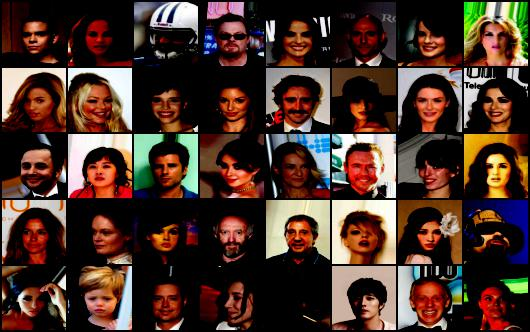
\includegraphics[width=75mm]{celeb_vae_ep_79_data}
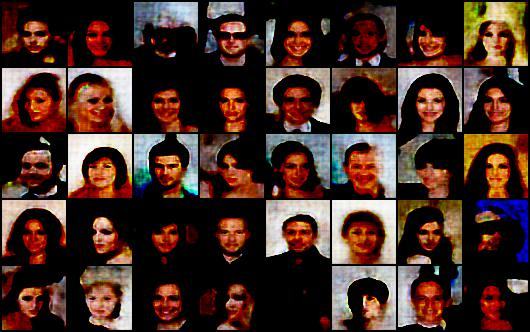
\includegraphics[width=75mm]{celeb_vae_ep_79_recon}
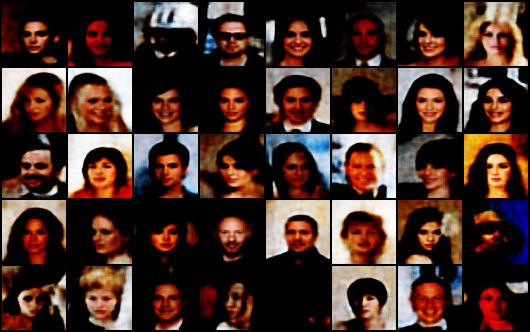
\includegraphics[width=75mm]{celeb_wae-mmd_ep_79_recon}
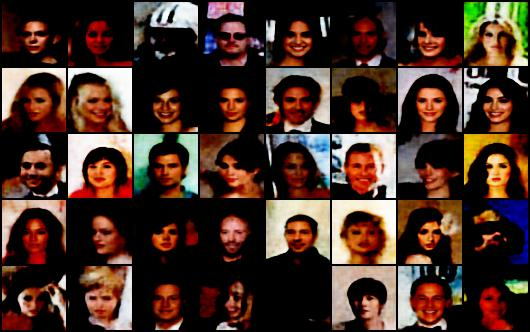
\includegraphics[width=75mm]{celeb_wae-gan_ep_79_recon}
\caption{Test CelebA reconstructions at epoch 80: original data (top left), VAE
         reconstructions (top right), WAE GAN reconstructions (bottom left), and
         WAE MDD reconstructions (bottom right).}
\label{Figure 2}
\end{figure}

\begin{figure}[htp]
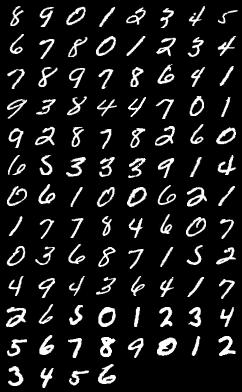
\includegraphics[width=36.5mm]{mnist_vae_ep_79_data}
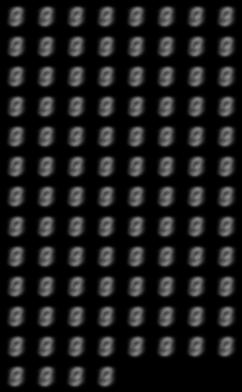
\includegraphics[width=36.5mm]{mnist_vae_ep_79_recon}
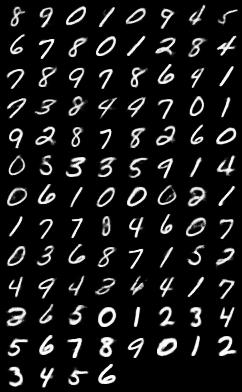
\includegraphics[width=36.5mm]{mnist_wae-gan_ep_79_recon}
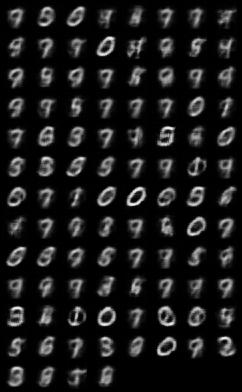
\includegraphics[width=36.5mm]{mnist_wae-mmd_ep_79_recon}
\caption{Test MNIST reconstructions at epoch 80:  using the VAE model.}
\label{Figure 3}
\end{figure}

\begin{table}[]
\centering
\caption{Blur and Fr\'echet Inception Distance (FID) Measures from CelebA dataset.}
\label{Table 1}
\begin{tabular}{lll}
        & Blur     & FID    \\
VAE     & 0.01947  & 0.1212 \\
WAE-GAN & 0.01151  & 0.1255 \\
WAE-MMD & 0.007089 & 0.1377
\end{tabular}
\end{table}

We note the following: \textbf{WAE-MMD} produces the lowest blur scores. In the
original paper, \textbf{WAE-GAN} produced the lowest blur scores. However, both
data types clearly produce less blurry images than \textbf{VAE}. In this sense
we have replicated the performance advantage of the \textbf{WAE} family proposed
by the authors. The results are less convincing for the Fr\'echet Inception
Distance (FID) scores. The VAE actually outperforms both \textbf{WAE} measures,
but the advantage isn't great and does not line up with the blur measure, nor
a qualitative analysis of the images. Furthermore, the distance values are much
smaller across the board than what was reported in the original paper, so we
suspect there may have been an error in our analysis. Briefly, we used the first
max-pooling features layer of the inception V3 network in all calculations. The
mean and standard deviations from the activations from this layer were then
used to compute the distance as:

$$ D D^T + trace(\sigma_1) + trace(\sigma_2) - 2 * \sqrt{\sigma_1 \sigma_2^T} $$

Where $D = \mu_1 - \mu_2$, $\mu_x$ represents the mean activation from image $x$,
and $\sigma_x$ represents the standard deviation of activations from image $x$. \\

We suspect that we would have gotten better results if we had taken the activation
from a lower layer of the inception V3 network. However, time constraints prevented
us from re-running these analyses. \\

The blur measure is simply calculated as the variance of the output of the
convolution of the reconstructed image with a laplacian filter. \\

Due to time constraints, we also did not replicate the latent-space traversal
analysis. We do not consider it a main result because it does little to compare
WAE with VAE, and we ran short on time due to having to debug the unstable
training of the MNIST data and the MMD-based analysis. We acknowledge that this
means we do not know for sure that the latent space learned by the WAE model is
continuous (as would be expected in a variational model), but given that
the other properties of the model were generally replicated, we assume this
property would hold as well.

\section{Discussion}

We are not critical of the experiments conducted considering the nature of the
result. Namely, they present a new kind of generative model, and then compare
the performance of this model using standard generative-model measures on stock
datasets. \\

We are critical that not many quantitative results are shown. Training curves
would have been welcome. There was also very little discussion of training
stability, which we found to be an extremely challenging aspect of this
replication. \\

We found multiple details of the implementation in the official source code
not reported in the paper. All references below refer to the official code: \\

\begin{center}
\textbf{https://github.com/tolstikhin/wae}
\end{center}

\begin{itemize}

    \item{For the reconstruction term of the loss (mean squared error), the
          authors \textbf{scale it by 5\%} (line 335 of wae.py). This is
          obviously crucial, as it weights the reconstruction term of the WAE
          loss (\verb|RECON + LAMBDA * PENALTY|) quite low compared to how they
          present the results in the paper. In our experiments, we tried using
          this scaling factor, lovingly called \verb|SCALEBULLSHIT|.}

    \item{For the MMD loss, the MMD value is accumulated times over different
          scales (line 294 of wae.py). We copied this implementation detail, but
          are unsure of it's relevance. Nonetheless, this implementation detail
          should be covered in the paper, or at the very least, be justified by
          a comment in the code.}

    \item{We found training to be rather unstable for the MMD method in
          particular. Training tended to collapse if the mean or standard
          deviation of the encoded data grew too large, which happened
          frequently for the MMD method. The authors combat this by clamping the
          sigma value during reparameterization between -50 and 50, which they
          do not comment on anywhere in the paper or code. We found this to be a
          crucial implementation detail, although it did not combat the issue
          entirely.}

    \item{In general, the balance between the reconstruction term and the
          Wasserstein penalty is extremely sensitive. The authors would have done
          well to have given a theoretical intuition as to which this might be true
          as well as practical recommendations to mitigate this issue when trying
          to implement the WAE yourself.}

\end{itemize}

Our major concern is the large difference in performance observed between using
\textbf{WAE-GAN}, which we found to be both stable and produce very good results,
and \textbf{WAE-MMD}, which we found to be extremely finicky and only sometimes
produce reasonable results after fastidious hyper-parameter fine-tuning. The
relationship between the reconstruction term and the WAE penalty is really evident
when using the MMD method, but the authors don't give any explanation as to why
either method would perform differently. Based on our experiments, we find it
very hard to believe that the authors did not encounter training instabilities
when using the MMD method, and would have liked to see the authors devote some
attention to explaining the real-world differences between these two approaches
to estimating the Wasserstein distance. \\

\bibliographystyle{plain}
\bibliography{references}

\end{document}
